% vim: set fileencoding=utf-8:
\documentclass{beamer}
\usepackage[utf8]{inputenc}
\usepackage[spanish]{babel}
\usepackage{fancybox}
\usepackage{graphics}
\usepackage{xcolor}
\usepackage{amsmath}

%\setbeamercovered{transparent}
%\includeonlyframes{current}

%\newcommand{\key}[1]{\framebox[1.8em]{\rule{0pt}{1em}#1}}
\newcommand{\placeholder}[1]{%
    \emph{$\langle$#1$\rangle$}%
}
\newcommand{\key}[1]{%
    \fcolorbox{black}{lightgray}{\rule[-.2em]{0pt}{1em}\makebox[1em][l]{#1}}%
}
\newcommand{\longkey}[1]{%
    \fcolorbox{black}{lightgray}{\rule[-.2em]{0pt}{1em}\makebox{#1}}%
}
\newcommand{\anykey}{%
    \fcolorbox{black}{red!75!green!50}{\rule[-.2em]{0pt}{1em}\makebox[1em][l]{}}%
}
\newcommand{\cmd}[1]{%
    \fcolorbox{black}{blue!75!green!50}{\rule[-.2em]{0pt}{1em}\makebox{\emph{#1}}}%
}
\newcommand{\cmdcount}{%
    \fcolorbox{black}{red!45!yellow!25}{\rule[-.2em]{0pt}{1em}\makebox{\emph{count}}}%
}
\newcommand{\typed}[1]{%
    \fcolorbox{blue!25!green!75}{blue!25!green!75}{\rule[-.2em]{0pt}{1em}\makebox{\texttt{#1}}}%
}
\newcommand{\cursor}[1]{%   TO BE IMPROVED
    \fcolorbox{black}{black}{\textcolor{white}{\hspace{-3.5pt}#1\hspace{-3.5pt}}}%
    %\fbox{$\!$#1$\!$}
}
\newcommand{\vimexample}[1]{%
    \fbox{\texttt{#1}}%
}

\newcommand{\foreign}{\textit}

\title {Edición eficiente de texto con Vim}
\author{Roberto Bonvallet \texttt{<rbonvall@inf.utfsm.cl>}}
\institute[UTFSM]{ Departamento de Informática \\
    Universidad Técnica Federico Santa María }
\date{20 de agosto de 2009}

\begin{document}

%\begin{frame}
%    \includegraphics[width=2in]{vim_putz1.jpg}
%    \includegraphics[width=2in]{vim_putz2.jpg}
%\end{frame}

\begin{frame}
    \titlepage
\end{frame}

\begin{frame}
    \only<1>{
        \begin{figure}[h]
            \begin{center}
                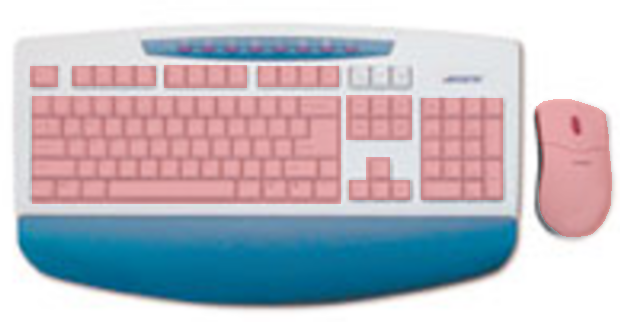
\includegraphics[width=4in]{kb-use-common}
            \end{center}
            \caption{Utilización frecuente del teclado y del ratón al
            acostumbrarse a un estilo de edición impuesto por un editor tipo
            Bloc de Notas}
            \label{fig:kb-use-common}
        \end{figure}
        
    }
    \only<2>{
        \begin{figure}[h]
            \begin{center}
                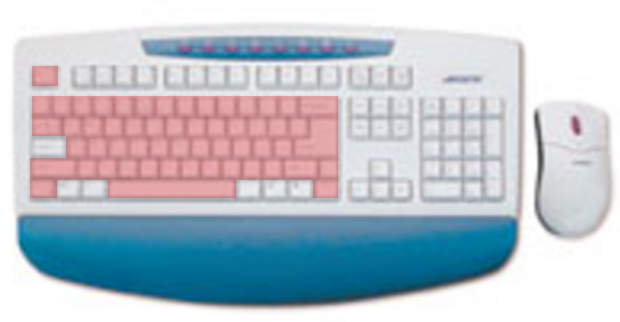
\includegraphics[width=4in]{kb-use-vim}
            \end{center}
            \caption{Utilización frecuente del teclado y del ratón al
            acostumbrarse a un estilo de edición impuesto por un editor tipo
            Vim}
            \label{fig:kb-use-common}
        \end{figure}
    }
\end{frame}

\begin{frame}
    \frametitle{Notación}
    \begin{itemize}
        \item \key{$x$}: la tecla $x$ presionada
        \item \anykey: una tecla cualquiera presionada
        \item \cmd{mov}: un movimiento realizado
        \item \cmdcount: un número tipeado antes de un comando
        \item \typed{lala}: el texto \textit{lala} tipeado tal cual
    \end{itemize}
\end{frame}

\begin{frame}
    \frametitle{Movimientos}
    \begin{itemize}
        \item (En modo normal) las teclas son comandos: no sirven para
            escribir texto.
        \item Los comandos, en general, son:
            \begin{itemize}
                \item movimientos
                \item operadores
            \end{itemize}
    \end{itemize}
\end{frame}

\begin{frame}
    \frametitle{Los comandos más paltosos del mundo}
    \begin{itemize}
        \item \key{.}: repite el último comando
        \item \key{u}: deshace el último comando (\foreign{undo})
    \end{itemize}
\end{frame}

\begin{frame}
    \frametitle{Movimientos}
    \key{h}, \key{j}, \key{k}, \key{l}
    \begin{itemize}
        \item Equivalentes a \key{$\leftarrow$}, \key{$\downarrow$},
            \key{$\uparrow$}, \key{$\rightarrow$}.
        \item Posición estratégica en el teclado:  permiten moverse sin
            levantar las manos del teclado.
        \item Mnemónicos:
            \begin{itemize}
                \item la \key{j} parece ser una letra que apunta hacia abajo
                \item la \key{k} parece ser una letra que apunta hacia arriba
                \item las teclas \key{h} y \key{l} están a la izquierda y a la derecha
                    de las anteriores en el teclado
            \end{itemize}
    \end{itemize}
\end{frame}

%  \item \key{\%}, \key{$*$}, \key{\#}
%  \item \key{`}\anykey, \key{'}\anykey
%  \item \longkey{Ctrl O}, \longkey{Ctrl I}
%  \item \key{H}, \key{M}, \key{L}

\begin{frame}
    \frametitle{Movimientos}
    \framesubtitle{Movimientos por palabra}
    \begin{itemize}
        \item \key{w}: avanza al comienzo de la palabra siguiente
            (\foreign{word})
        \item \key{b}: retrocede al comienzo de una palabra
            (\foreign{beginning})
        \item \key{e}: avanza al final de la palabra
            (\foreign{end})
        \item Se considera como palabra cualquier secuencia de letras, dígitos y
            guiones de subrayado.
        \item \key{W}, \key{B} y \key{E} consideran como palabra cualquier
            secuencia de caracteres separados por espacios.
    \end{itemize}
\end{frame}

\begin{frame}
    \frametitle{Movimientos}
    \framesubtitle{Movimientos del contenido de la pantalla}
    \begin{itemize}
        \item \longkey{Ctrl F}: desplaza una página hacia adelante
            (\foreign{forwards})
        \item \longkey{Ctrl B}: desplaza una página hacia atras
            (\foreign{backwards})
        \item \longkey{Ctrl E}: desplaza una línea hacia arriba
            (\foreign{extra lines})
        \item \longkey{Ctrl Y}: desplaza una línea hacia abajo
        \item \key{z}\key{z}: deja la línea actual en el centro de la pantalla
    \end{itemize}
\end{frame}

\begin{frame}
    \frametitle{Movimientos}
    \framesubtitle{Movimientos relativos a la pantalla}
    \begin{itemize}
        \item \key{H}: mueve el cursor a la primera línea de la pantalla
            (\foreign{higher})
        \item \key{M}: mueve el cursor a la línea del medio de la pantalla
            (\foreign{middle})
        \item \key{L}: mueve el cursor a la última línea de la pantalla
            (\foreign{lower})
    \end{itemize}
\end{frame}

\begin{frame}
    \frametitle{Movimientos}
    \framesubtitle{Movimientos por línea}
    \begin{itemize}
        \item \key{g}\key{g}: mueve el cursor a la primera línea del archivo
            %(\foreign{go, go!})
        \item \key{G}: mueve el cursor a la última línea del archivo
            %(\foreign{GO!})
        \item \cmdcount\key{g}\key{g}: mueve  el cursor a la línea \cmdcount.
        \item \cmdcount\key{G}: ídem
        \item \cmdcount\key{\%}: mueve el cursor a la línea correspondiente al
            \cmdcount\ porciento de las líneas del archivo
    \end{itemize}
\end{frame}

\begin{frame}
    \frametitle{Movimientos}
    \framesubtitle{Movimientos por objetos de texto}
    \begin{itemize}
        \item \key{$($}, \key{$)$}: movimiento por oración
        \item \key{$\{$}, \key{$\}$}: movimiento por párrafo
    \end{itemize}
\end{frame}

\begin{frame}
    \frametitle{Movimientos}
    \framesubtitle{Movimientos en una línea}
    \begin{itemize}
        \item \key{0}:  principio de la línea
        \item \key{\$}:  final de la línea
        \item \key{$\wedge$}: primer caracter no blanco
        \item \key{f}\anykey: próxima ocurrencia de \anykey{} en la línea
            (\foreign{find})
        \item \key{F}\anykey: anterior ocurrencia de \anykey{} en la línea
        \item \key{t}\anykey: un caracter antes del próximo \anykey{}
            (\foreign{`til})
        \item \key{T}\anykey: un caracter después del anterior \anykey{}
        \item \key{;}: repite el último \key{f}, \key{F}, \key{t} o \key{T}.
    \end{itemize}
\end{frame}

\begin{frame}
    \frametitle{Movimientos}
    \framesubtitle{Otros movimientos}
    \begin{itemize}
        \item \key{\%}: busca el paréntesis apareado con el que está bajo el
            cursor 
            \begin{itemize}
                \item funciona para
                    \texttt{()},
                    \texttt{\{\}},
                    \texttt{[]},
                    \texttt{\#if \#endif},
                    \texttt{/* */}.
            \end{itemize}
        \item \longkey{Ctrl O}: retorna a la posición anterior antes del último
            movimiento (\foreign{old position})
        \item \longkey{Ctrl I}: deshace el \longkey{Ctrl O}
    \end{itemize}
\end{frame}

\begin{frame}
    \frametitle{Ejemplos de movimientos en una línea}

    \only<1>{\vimexample{Dábale arroz a la \cursor{z}orra el abad.}}
    \only<2>{\vimexample{Dábale arroz a \cursor{l}a zorra el abad.}}
    \only<3>{\vimexample{\cursor{D}ábale arroz a la zorra el abad.}}
    \only<4>{\vimexample{Dábale arro\cursor{z} a la zorra el abad.}}
    \only<5>{\vimexample{Dábale arroz a \cursor{l}a zorra el abad.}}
    \only<6>{\vimexample{Dábale arroz a la zorra el abad\cursor{.}}}
    \only<7>{\vimexample{Dábale arroz a l\cursor{a} zorra el abad.}}
    \only<8>{\vimexample{Dábale arroz a la \cursor{z}orra el abad.}}
    \\
    \uncover<2->{\key{b}}
    \uncover<3->{\key{0}}
    \uncover<4->{\key{f}\key{z}}
    \uncover<5->{\key{2}\key{w}}
    \uncover<6->{\key{\$}}
    \uncover<7->{\key{1}\key{5}\key{h}}
    \uncover<8->{\key{;}}
\end{frame}




\begin{frame}
    \frametitle{Operaciones básicas}
    \begin{itemize}
        \item \key{$\sim$}:  cambia minúsculas/mayúsculas del caracter bajo el
            cursor
        \item \key{x}:  suprime el caracter bajo el cursor
        \item \key{X}:  suprime el caracter anterior al cursor
        \item \key{r}\anykey:  reemplaza el caracter bajo el cursor por \anykey
        %\item \key{m}\anykey
        \item \longkey{Ctrl A}:  incrementa el número bajo el cursor
            (\foreign{add})
        \item \longkey{Ctrl X}:  decrementa el número bajo el cursor
            (\foreign{extract})
        %\item \key{u}: deshace el último comando (\foreign{undo})
        %\item \key{.}: repite el último comando
    \end{itemize}
\end{frame}

\begin{frame}
    \frametitle{Ejemplos de operaciones básicas}

    \only<1>{\vimexample{hola, te invito a m\cursor{i} fiezta de 11 años.}}
    \only<2>{\vimexample{\cursor{h}ola, te invito a mi fiezta de 11 años.}}
    \only<3>{\vimexample{H\cursor{o}la, te invito a mi fiezta de 11 años.}}
    \only<4>{\vimexample{Hola, te invito a mi fie\cursor{z}ta de 11 años.}}
    \only<5>{\vimexample{Hola, te invito a mi fie\cursor{s}ta de 11 años.}}
    \only<6>{\vimexample{Hola, te invito a mi fiesta de \cursor{1}1 años.}}
    \only<7>{\vimexample{Hola, te invito a mi fiesta de \cursor{1}5 años.}}
    \only<8>{\vimexample{Hola, te invito a mi fiesta de \cursor{1}9 años.}}
    \only<9>{\vimexample{Hola, te invito a mi fiesta de \cursor{1}5 años.}}
    \\
    \uncover<2->{\key{0}}
    \uncover<3->{\key{$\sim$}}
    \uncover<4->{\key{f}\key{z}}
    \uncover<5->{\key{r}\key{s}}
    \uncover<6->{\key{2}\key{w}}
    \uncover<7->{\key{4}\longkey{Ctrl A}}
    \uncover<8->{\key{.}}
    \uncover<9->{\key{u}}
\end{frame}

%%%%%%%%%%%%%%%% PRUEBA TEST E %%%%%%%%%%%%%%%
\newcommand{\exampleline}[1]{\makebox[28em][l]{\texttt{#1}}}
\newcommand{\examplelines}[1]{\fbox{\parbox{28em}{#1}}}
\begin{frame}[fragile,label=current]
    \frametitle{Otro ejemplo más}
    \only<1>{\examplelines{
        \exampleline{En un lugar de la marcha}
        \exampleline{de cuyo nom\cursor{b}re no quiero hacordarme}
    }}
    \only<2>{\examplelines{
        \exampleline{En un lugar\cursor{ }de la marcha}
        \exampleline{de cuyo nombre no quiero hacordarme}
    }}
    \only<3>{\examplelines{
        \exampleline{En un lugar de la \cursor{m}archa}
        \exampleline{de cuyo nombre no quiero hacordarme}
    }}
    \only<4>{\examplelines{
        \exampleline{En un lugar de la M\cursor{a}rcha}
        \exampleline{de cuyo nombre no quiero hacordarme}
    }}
    \only<5>{\examplelines{
        \exampleline{En un lugar de \cursor{l}a Marcha}
        \exampleline{de cuyo nombre no quiero hacordarme}
    }}
    \only<6>{\examplelines{
        \exampleline{En un lugar de L\cursor{a} Marcha}
        \exampleline{de cuyo nombre no quiero hacordarme}
    }}
    \only<7>{\examplelines{
        \exampleline{En un lugar de la Ma\cursor{r}cha}
        \exampleline{de cuyo nombre no quiero hacordarme}
    }}
    \only<8>{\examplelines{
        \exampleline{En un lugar de la Ma\cursor{n}cha}
        \exampleline{de cuyo nombre no quiero hacordarme}
    }}
    \only<9>{\examplelines{
        \exampleline{En un lugar de la Mancha}
        \exampleline{de cuyo nombre no qu\cursor{i}ero hacordarme}
    }}
   \only<10>{\examplelines{
        \exampleline{En un lugar de la Mancha}
        \exampleline{de cuyo nombre no quiero \cursor{h}acordarme}
    }}
   \only<11>{\examplelines{
        \exampleline{En un lugar de la Mancha}
        \exampleline{de cuyo nombre no quiero \cursor{a}cordarme}
    }}
   \only<12,14>{\examplelines{
        \exampleline{En un lugar de la Mancha}
        \exampleline{de cuyo nombre no quiero acordarm\cursor{e}}
    }}
   \only<13>{\examplelines{
        \exampleline{En un lugar de la Mancha}
        \exampleline{de cuyo nombre no quiero acordarme\cursor{h}}
    }}
    \\
    \uncover <2->{\key{k}}
    \uncover <3->{\key{3}\key{w}}
    \uncover <4->{\key{$\sim$}}
    \uncover <5->{\key{F}\key{l}}
    \uncover <6->{\key{.}}
    \uncover <7->{\key{f}\key{r}}
    \uncover <8->{\key{r}\key{n}}
    \uncover <9->{\key{j}}
    \uncover <10->{\key{f}\key{h}}
    \uncover <11->{\key{x}}
    \uncover<12->{\key{\$}}
    \uncover<13->{\key{p}}
    \uncover<14->{\key{u}}
\end{frame}

\begin{frame}
    \frametitle{¿Cómo comenzar a escribir?}
    \begin{itemize}
        \item \key{i}:  comienza a escribir antes del cursor (\foreign{insert})
        \item \key{s}:  comienza a escribir encima del cursor
            (\foreign{substitute})
        \item \key{a}:  comienza a escribir después del cursos
            (\foreign{append})
        \item \key{I}:  comienza a escribir al principio de la línea
        \item \key{A}:  comienza a escribir al final de la línea
        \item \key{o}:  comienza a escribir en una línea nueva a continuación
            de la actual (\foreign{open new line})
        \item \key{O}:  comienza a escribir en una línea nueva antes de la
            actual
        \item<2> Al terminar de escribir, presionar \longkey{Esc}
    \end{itemize}
\end{frame}

\begin{frame}
    \frametitle{Comandos paltosos en modo inserción}
    \begin{itemize}
        \item \longkey{Ctrl H}, \longkey{Ctrl U}: borra el caracter
            anterior/hasta el final de la línea
        \item \longkey{Ctrl T}, \longkey{Ctrl D}: indenta/dedenta la línea
            actual
        \item \longkey{Ctrl Y}, \longkey{Ctrl E}: copia el caracter arriba/abajo
            del cursor
        \item \longkey{Ctrl P}, \longkey{Ctrl N}: completa la palabra que se
            está escribiendo
        \item \longkey{Ctrl X}\longkey{Ctrl F}, \longkey{Ctrl X}\longkey{Ctrl L}
    \end{itemize}
\end{frame}

\begin{frame}
    \frametitle{Operadores}
    \begin{itemize}
        \item \key{c}\cmd{mov}, \key{d}\cmd{mov}, \key{y}\cmd{mov}
        \item \key{g}\key{$\sim$}\cmd{mov}, \key{g}\key{u}\cmd{mov},
            \key{g}\key{U}\cmd{mov}
        \item \key{!}\cmd{mov}, \key{=}\cmd{mov}, \key{g}\key{q}\cmd{mov},
            \key{g}\key{?}\cmd{mov}
        \item \key{$>$}\cmd{mov}, \key{$<$}\cmd{mov}
        \item Comando repetido se aplica a la línea actual
    \end{itemize}
\end{frame}

\begin{frame}
    \frametitle{Ejemplos de uso de operadores}
    \begin{itemize}
        \item \key{c}\key{w}\typed{lala}\longkey{Esc}
        \item \key{b}\key{y}\key{\$}\key{0}\key{P}
        \item \key{d}\key{d}\key{p} 
        \item \key{g}\key{g}\key{O}\typed{\#include
            "lala.h"}\longkey{Esc}\longkey{Ctrl O}
        \item \longkey{Ctrl A}\key{2}\key{j}\key{.}
        \item \key{I}\typed{/$*$}\longkey{Esc}\key{A}\typed{$*$/}\longkey{Esc}
        \item \key{F}\key{$\{$}\key{d}\key{\%}\key{20}\key{k}\key{p}
    \end{itemize}
\end{frame}

\begin{frame}
    \frametitle{Ejemplos de operadores con pseudomovimientos}
    \begin{itemize}
        \item \key{d}\key{i}\key{w}
        \item \key{g}\key{q}\key{a}\key{p}
        \item \key{c}\key{i}\key{$\}$}\typed{Blah blah}\longkey{Esc}
    \end{itemize}
\end{frame}

\begin{frame}
    \frametitle{Modo visual}
    \begin{itemize}
        \item \key{v}: selección por caracteres
        \item \key{V}: selección por líneas
        \item \longkey{Ctrl V}: selección en bloque
    \end{itemize}
\end{frame}

\begin{frame}
    \frametitle{Modo ex (línea de comandos)}
    \begin{itemize}
        \item \key{:}\typed{e \placeholder{archivo}}\longkey{Enter}
        \item \key{:}\typed{w \placeholder{archivo}}\longkey{Enter}
        \item \key{:}\typed{w}\longkey{Enter}
        \item \key{:}\typed{3,\$w}\longkey{Enter}
        \item \key{:}\typed{wq}\longkey{Enter}
        \item \key{:}\typed{r  \placeholder{archivo}}\longkey{Enter}
        \item \key{:}\typed{r! \placeholder{comando}}\longkey{Enter}
    \end{itemize}
\end{frame}

\begin{frame}
    \frametitle{Modo ex, segunda parte}
    \begin{itemize}
        \item \key{:}\typed{.,+5d}\longkey{Enter}
        \item \key{:}\typed{2,\$normal 02fñx\$}\longkey{Enter}
        \item
            \key{:}\typed{\%s/textbf/emph/gc}\longkey{Enter}
        \item \key{:}\typed{g/item/d}\longkey{Enter}
            \key{:}\typed{g/$\wedge$[ ]$*$\#/normal A \#XXX}\longkey{Enter}
        \item \key{:}\typed{1,.j}\longkey{Enter}
    \end{itemize}
\end{frame}

\begin{frame}
    \frametitle{Búsqueda}
    \begin{itemize}
        \item \key{/}\typed{\placeholder{patrón}}\longkey{Enter}: busca el
            patrón hacia adelante
        \item \key{?}\typed{\placeholder{patrón}}\longkey{Enter}: busca el
            patrón hacia atrás
        \item \key{n}, \key{N}: busca próxima/anterior ocurrencia de la última
            búsqueda
        \item \key{$*$}, \key{\#}: busca próxima/anterior ocurrencia de la
            palabra bajo el cursor
    \end{itemize}
\end{frame}

\begin{frame}
    \frametitle{Mapeos y abreviaciones}
    \begin{itemize}
        \item \key{:}\typed{map \placeholder{secuencia} \placeholder{secuencia}}\longkey{Enter}
        \item \key{:}\typed{imap \placeholder{secuencia} \placeholder{secuencia}}\longkey{Enter}
        \item \key{:}\typed{noremap \placeholder{secuencia} \placeholder{secuencia}}\longkey{Enter}
        \item \key{:}\typed{iabbrev \placeholder{abreviación} \placeholder{texto}}\longkey{Enter}
    \end{itemize}
\end{frame}

\begin{frame}
    \frametitle{Macros}
    \begin{itemize}
        \item \key{q}\anykey: comienza a grabar una macro en el registro \anykey
        \item \key{@}\anykey: ejecuta la macro grabada en \anykey
        \item \key{@}\key{@}: ejecuta la última macro ejecutada
    \end{itemize}
\end{frame}

\begin{frame}
    \frametitle{Ventanas}
    \begin{itemize}
        \item \key{:}\typed{new}\longkey{Enter}
        \item \key{:}\typed{vnew}\longkey{Enter}
        \item \longkey{Ctrl W}\key{n}
        \item \longkey{Ctrl W}\longkey{Ctrl W}
        \item \longkey{Ctrl W}\key{j},\longkey{Ctrl W}\key{l}
        \item \longkey{Ctrl W}\key{J},\longkey{Ctrl W}\key{L}
    \end{itemize}
\end{frame}

\end{document}
